\chapter{Results}
\label{chap:results}

In the \MFM analysis the data in all 25 analysis categories (11 at 7~TeV, 14 at 8~TeV) is simultaneously fitted with a background and signal component. The background normalisation and shape parameters (which includes the different function choices) are completely free floating, i.e.~there is no constraint on their values. The signal shape is allowed to vary according to the systematic uncertainties described in Sec.~\ref{sec:systematics}. The parametrisation of the signal yield is such that, although the overall rate is floating, the fraction in each category is required to match the prediction of a \SM Higgs boson (modulo the nuisance parameters). For some of the coupling measurements these signal constraints are relaxed such that the signal strength through bosonic production modes (\VBF,\VH) and through fermionic production modes (\ggH,\ttH) are allowed to float independently. 

Where appropriate the results of the \MFM and \SMVA are shown next to each other. As the \SMVA is a cross-check to the background model and categorisation scheme, only results on exclusion power, observation significance and signal strength measurement are provided for the \SMVA. The results of couplings measurements and compatibility across channels and production mechanisms are shown only for the \MFM.

The first section shows the results of the best fit signal plus background model to data. In the second section the results of the statistical hypothesis tests are shown: the exclusion limit of a \SM Higgs boson and the local probability of a signal-like background fluctuation ($p$-value test). These establish an independent discovery of a Higgs-like resonance near 125~GeV. The last two sections focus on understanding some of the properties of the observed state with respect to the \SM expectation: measurements of its mass and coupling parameters and hypothesis tests comparing various spin models to the data.

\section{Best fit model to data}

This section shows the best fit result of the signal plus background model when floating both the signal strength, $\mu=\musm$, and the signal position, $\mH$, whilst fitting simultaneously across all of the analysis categories using the nominal \MFM analysis. Figures~\ref{fig:bfres1}-\ref{fig:bfres5} show the best fit result in each analysis category. Figures~\ref{fig:sbfit_unw} and~\ref{fig:sbfit_w} show the fully inclusive distribution with the full signal plus background model and a data-background residual underneath. It is apparent from these two plots that a substantial signal is observed near $\mH=125$~GeV.

\begin{figure}
  \vspace{-1cm}
  \includegraphics[width=0.49\textwidth]{results/plots/mgg-cats/mgg_mva_nosub_ch1_cat0_7TeV.pdf}
  \includegraphics[width=0.49\textwidth]{results/plots/mgg-cats/mgg_mva_nosub_ch1_cat1_7TeV.pdf}
  \includegraphics[width=0.49\textwidth]{results/plots/mgg-cats/mgg_mva_nosub_ch1_cat2_7TeV.pdf}
  \includegraphics[width=0.49\textwidth]{results/plots/mgg-cats/mgg_mva_nosub_ch1_cat3_7TeV.pdf}
  \includegraphics[width=0.49\textwidth]{results/plots/mgg-cats/mgg_mva_nosub_ch1_cat4_7TeV.pdf}
  \includegraphics[width=0.49\textwidth]{results/plots/mgg-cats/mgg_mva_nosub_ch1_cat5_7TeV.pdf}
  \caption[The diphoton invariant mass distribution in data with the best fit signal plus background overlaid for the untagged and dijet tagged categories in the 8~TeV dataset]{The diphoton invariant mass distribution in data (black points) with the best fit signal plus background overlaid (solid red line), including the background only component (dashed red line) and the uncertainty on the background shape (yellow and green bands). Shown for the untagged and dijet categories in the 7~TeV dataset.}
  \label{fig:bfres1}
\end{figure}

\begin{figure}
  \vspace{-1cm}
  \includegraphics[width=0.49\textwidth]{results/plots/mgg-cats/mgg_mva_nosub_ch1_cat6_7TeV.pdf}
  \includegraphics[width=0.49\textwidth]{results/plots/mgg-cats/mgg_mva_nosub_ch1_cat7_7TeV.pdf}
  \includegraphics[width=0.49\textwidth]{results/plots/mgg-cats/mgg_mva_nosub_ch1_cat8_7TeV.pdf}
  \includegraphics[width=0.49\textwidth]{results/plots/mgg-cats/mgg_mva_nosub_ch1_cat10_7TeV.pdf}
  \includegraphics[width=0.49\textwidth]{results/plots/mgg-cats/mgg_mva_nosub_ch1_cat9_7TeV.pdf}
  \caption[The diphoton invariant mass distribution in data with the best fit signal plus background overlaid for the \acs{VH} and \acs{ttH}-tagged categories in the 8~TeV dataset]{The diphoton invariant mass distribution in data (black points) with the best fit signal plus background overlaid (solid red line), including the background only component (dashed red line) and the uncertainty on the background shape (yellow and green bands). Shown for the \VH and \ttH-tagged categories in the 7~TeV dataset.}
  \label{fig:bfres2}
\end{figure}

\begin{figure}
  \vspace{-1cm}
  \includegraphics[width=0.49\textwidth]{results/plots/mgg-cats/mgg_mva_nosub_ch2_cat0_8TeV.pdf}
  \includegraphics[width=0.49\textwidth]{results/plots/mgg-cats/mgg_mva_nosub_ch2_cat1_8TeV.pdf}
  \includegraphics[width=0.49\textwidth]{results/plots/mgg-cats/mgg_mva_nosub_ch2_cat2_8TeV.pdf}
  \includegraphics[width=0.49\textwidth]{results/plots/mgg-cats/mgg_mva_nosub_ch2_cat3_8TeV.pdf}
  \includegraphics[width=0.49\textwidth]{results/plots/mgg-cats/mgg_mva_nosub_ch2_cat4_8TeV.pdf}
  \includegraphics[width=0.49\textwidth]{results/plots/mgg-cats/mgg_mva_nosub_ch2_cat5_8TeV.pdf}
  \caption[The diphoton invariant mass distribution in data with the best fit signal plus background overlaid for the untagged and dijet 0 categories in the 8~TeV dataset]{The diphoton invariant mass distribution in data (black points) with the best fit signal plus background overlaid (solid red line), including the background only component (dashed red line) and the uncertainty on the background shape (yellow and green bands). Shown for the untagged and dijet 0 categories in the 8~TeV dataset.}
  \label{fig:bfres3}
\end{figure}

\begin{figure}
  \vspace{-1cm}
  \includegraphics[width=0.49\textwidth]{results/plots/mgg-cats/mgg_mva_nosub_ch2_cat6_8TeV.pdf}
  \includegraphics[width=0.49\textwidth]{results/plots/mgg-cats/mgg_mva_nosub_ch2_cat7_8TeV.pdf}
  \includegraphics[width=0.49\textwidth]{results/plots/mgg-cats/mgg_mva_nosub_ch2_cat8_8TeV.pdf}
  \includegraphics[width=0.49\textwidth]{results/plots/mgg-cats/mgg_mva_nosub_ch2_cat9_8TeV.pdf}
  \includegraphics[width=0.49\textwidth]{results/plots/mgg-cats/mgg_mva_nosub_ch2_cat10_8TeV.pdf}
  \includegraphics[width=0.49\textwidth]{results/plots/mgg-cats/mgg_mva_nosub_ch2_cat13_8TeV.pdf}
  \caption[The diphoton invariant mass distribution in data with the best fit signal plus background overlaid for the dijet 1,2 and \acs{VH}-tagged categories in the 8~TeV dataset]{The diphoton invariant mass distribution in data (black points) with the best fit signal plus background overlaid (solid red line), including the background only component (dashed red line) and the uncertainty on the background shape (yellow and green bands). Shown for the dijet 1,2 and \VH-tagged categories in the 8~TeV dataset.}
  \label{fig:bfres4}
\end{figure}

\begin{figure}
  \vspace{-1cm}
  \includegraphics[width=0.49\textwidth]{results/plots/mgg-cats/mgg_mva_nosub_ch2_cat11_8TeV.pdf}
  \includegraphics[width=0.49\textwidth]{results/plots/mgg-cats/mgg_mva_nosub_ch2_cat12_8TeV.pdf}
  \caption[The diphoton invariant mass distribution in data with the best fit signal plus background overlaid for the \acs{ttH}-tagged categories in the 8~TeV dataset]{The diphoton invariant mass distribution in data (black points) with the best fit signal plus background overlaid (solid red line), including the background only component (dashed red line) and the uncertainty on the background shape (yellow and green bands). Shown for the \ttH-tagged categories in the 8~TeV dataset.}
  \label{fig:bfres5}
\end{figure}

\begin{figure}
  \includegraphics[width=0.7\textwidth]{results/plots/mgg_mva_fullrange_combcat78TeV_unweighted.pdf}
  \caption[The unweighted diphoton invariant mass distribution for all analysis events in data with the combined best fit signal plus background model overlaid]{The diphoton invariant mass distribution for all analysis events in the range $100<\mgg<180$~GeV in data (black points) with the combined best fit signal plus background model overlaid (solid red line), including the background only component (dashed red line) and the uncertainty on the background shape (yellow and green bands). The data minus background residual is shown at the bottom.}
  \label{fig:sbfit_unw}
\end{figure}

\begin{figure}
  \includegraphics[width=0.85\textwidth]{results/plots/mgg_mva_110_150_combcat78TeV_weighted.pdf}
  \caption[The S/(S+B) weighted diphoton invariant mass distribution for all analysis events in data with the combined best fit signal plus background model overlaid]{The diphoton invariant mass distribution for all analysis events in the analysis search range $110<\mgg<150$~GeV in data (black points) with the combined best fit signal plus background model overlaid (solid red line), including the background only component (dashed red line) and the uncertainty on the background shape (yellow and green bands). In this plot the data, signal and background models in each analysis category are given a weight according to the expected S/(S+B) ratio in $\pm\sigeff$ of the best fit mass. The plot is then normalised such that the integral under the signal peak gives the same number of events as the non-weighted equivalent. This plot helps to show the fitted signal by upweighting categories with higher sensitivity. The data minus background residual is shown at the bottom.}
  \label{fig:sbfit_w}
\end{figure}

\section{Exclusion limits and $p$-value}

The exclusion limit for a \SM Higgs boson is shown in Fig.~\ref{fig:res_exclusion} for the \MFM analysis (left) and the \SMVA analysis (right) for the combined 7 and 8~\TeV dataset. In this figure, the test statistic used is the one defined in Eq.~\ref{eq:teststat}. The signal position, \mH, is set to a given value and the signal strength, $\mu$, is altered until the required value of $CL_{s}$, in this case 5\%, is obtained. This allows determination of the signal strength excluded at 95\%~C.L.~for a given signal mass. This plot shows the cross section, relative to the \SM prediction, excluded at 95\% confidence using the $CL_{s}$ method as a function of the Higgs mass, \mH, in steps of 1~GeV. This has become a standard plot for Higgs searches and aims to determine what cross sections can be ruled out for a Higgs boson at a given mass. The black dashed line, with the green and yellow bands, represents the expected exclusion, and the associated $\pm1\sigma$ and $\pm2\sigma$ error, if exactly the mean of the null hypothesis is observed. The solid black line represents the actual observation in data. For values of \mH where the solid black line falls below the solid red line at 1, the \SM Higgs boson is excluded at a confidence level of 95\% or higher. It is clear that a \SM Higgs boson is excluded at all values of \mH apart from near 125~GeV where there is a large excess (well above the $2\sigma$ band).
It can be seen that both the nominal \MFM analysis and the cross-check \SMVA have similar exclusion power (shown by the position of the dashed line and coloured bands) and a similar observation.

\begin{figure}
  \includegraphics[width=0.49\textwidth]{results/plots/mva_limit.pdf}
  \includegraphics[width=0.49\textwidth]{results/plots/sideband_limit.pdf}
  \caption[The expected and observed exclusion limits for a \acs{SM} Higgs boson at 95\% confidence level]{The expected and observed exclusion limits for a \SM Higgs boson at 95\% confidence level. The dashed line shows the expected exclusion if exactly the mean of the null hypothesis is observed with its error at $1\sigma$ (green) and $2\sigma$ (yellow). The solid black line shows the observed exclusion. The results are shown for the nominal \MFM analysis (left) and the cross-check \SMVA (right) when combining both the 7 and 8~\TeV datasets. A \SM Higgs boson is disfavoured everywhere, at 95\% confidence level or higher, apart from where there is a large excess around 125~\GeV.}
  \label{fig:res_exclusion}
\end{figure}

In order to quantify the significance of this excess the test statistic defined in Eq.~\ref{eq:pvalue} is used. This is employed to determine the probability, the local $p$-value, that the background can fluctuate to give an observed signal by comparing the likelihoods for the null and alternate hypothesis at a given Higgs mass. The observed local $p$-value is shown as a function of the hypothesised Higgs mass, \mH, in Fig.~\ref{fig:res_pvalue} for both the 7~\TeV (blue line) and 8~\TeV (red line) datasets separately and the combination (black line). It is clear there is a significant excess in both subsets of data at approximately the same mass and the quantity of the excess is apparent in both the \MFM and \SMVA analyses. The local $p$-value for the \MFM using the combined 7 and 8~\TeV datasets at $\mH=124.7$~\GeV (the mass with the most significant excess) equates to a significance of 5.7$\sigma$ where 5.2$\sigma$ is the expectation for a \SM Higgs boson. This constitutes a standalone discovery of a Higgs-like resonance around 125~\GeV.

\begin{figure}
  \includegraphics[width=0.49\textwidth]{results/plots/mva_pval.pdf}
  \includegraphics[width=0.49\textwidth]{results/plots/sideband_pval_fix.pdf}
  \caption[The expected and observed local $p$-value to reject the background hypothesis]{The expected (dashed lines) and observed (solid lines) local $p$-value to reject the background only hypothesis as a function of the hypothesised Higgs mass, \mH. The 7~\TeV (blue lines) and 8~\TeV (red lines) results are show separately along with the combination (black lines). The results are shown for the nominal \MFM analysis (left) and the cross-check \SMVA (right). The observed $p$-value in the \MFM at the most significant point is 5.7$\sigma$ ($\mH=124.7$~\GeV) given a \SM expectation of $5.2\sigma$.}
  \label{fig:res_pvalue}
\end{figure}

\section{Measurement of physical parameters}

The best fit value of the signal strength modifier, $\mu=\musm$, is shown as a function of the hypothesis Higgs mass, \mH, in Fig.~\ref{fig:res_mumh} for the combined 7 and 8~\TeV dataset. As expected this follows very closely the shape of the observed exclusion in Fig.~\ref{fig:res_exclusion} and shows that the observed boson is very compatible with a \SM Higgs, i.e.~the observed value of $\mu$ is within $1\sigma$ of the \SM expectation, $\mu=1$. 

\begin{figure}
  \includegraphics[width=0.49\textwidth]{results/plots/mva_greenband.pdf}
  \includegraphics[width=0.49\textwidth]{results/plots/sideband_greenband.pdf}
  \caption[The observed best fit value of the signal strength modifier $\mu$]{The observed best fit value of the signal strength modifier, $\mu=\musm$, as a function of the hypothesised Higgs mass \mH when using the combined 7 and 8~\TeV datasets. The $\pm1\sigma$ error band is shown as the green band. Results are shown for the nominal \MFM analysis (left) and the cross-check \SMVA analysis (right).}
  \label{fig:res_mumh}
\end{figure}

Figure~\ref{fig:res_muscan} shows the one dimensional \NLL scan of $\mu$ when the Higgs mass \mH is profiled. The hypothesis mass, \mH, is left floating in the fit as there is no \textit{a priori} knowledge of its value. One can see that the results are very consistent between the \MFM (left) and the \SMVA (right). There is some distance between the measurement made using the 7~\TeV dataset (blue line) and the 8~\TeV dataset (red line) but they are consistent at $<2\sigma$ level and it is quite reasonable to imagine an upward fluctuation in the data at 7~\TeV and a downward fluctuation at 8~\TeV. When combining the two datasets the best fit value comes out very close to the \SM expectation of $\mu=1$ so certainly an interesting area for future measurements with more data in the \Hgg channel is where this value goes. The best fit values of $\musm$ with their errors (and the mass at which the best fit is found) are summarised for each of the datasets using the \MFM analysis in Table~\ref{tab:res_mu}. The overall best fit of the signal strength is $\sigma/\sigma_{SM} = 1.14^{+0.26}_{-0.23} \;\Bigl[\;^{+0.21}_{-0.21} \mathrm{(stat)} ^{+0.13}_{-0.09} \mathrm{(theory)} ^{+0.09}_{-0.05} \mathrm{(syst)} \Bigr]$.

\begin{figure}
  \includegraphics[width=0.49\textwidth]{results/plots/mva_mu_scan.pdf}
  \includegraphics[width=0.49\textwidth]{results/plots/sideband_mu_scan.pdf}
  \caption[The 1D \NLL scan of the signal strength modifier $\mu$]{The one dimensional \NLL scan of the signal strength modifier, $\mu=\musm$, when the hypothesis Higgs mass, \mH, is profiled in the fit. The results are shown for the 7~\TeV (blue), the 8~\TeV (red) and combined (black) datasets using the \MFM analysis (left) and the \SMVA analysis (right). The observed best fit value for the nominal \MFM analysis is $\musm=1.14^{+0.26}_{-0.23}$.}
  \label{fig:res_muscan}
\end{figure}

\begin{table}
    \caption[The values of the best fit signal strength, $\musm$, when \mH is profiled, for the 7~TeV, 8~TeV and combined datasets]{\label{tab:res_mu} The values of the best fit signal
      strength, $\musm$, when \mH is profiled, for the 7~\TeV, 8~\TeV, and combined datasets. 
      The value of \mH\ at which the best fit occurs is also given.
      }
  \begin{center}
    \begin{tabular}{l c c}
      & $\musm$  & $\mH$ (GeV)       \\  
      \hline
      \hline
      7 TeV  & $2.22^{+0.60}_{-0.54}$ & 124.2  \\ 
      8 TeV  & $0.90^{+0.25}_{-0.23}$ & 124.9  \\ \hline
      7 + 8 TeV & $1.14^{+0.26}_{-0.23}$ & 124.7  \\ 
    \end{tabular}
    \end{center}
\end{table}

The following measurements focus on the properties of the observed signal and are consequently only shown for the \MFM analysis. The two most important physical parameters to measure in the signal are the overall rate, $\mu$, and the mass, \mH. We have seen the one dimensional \NLL scan of the signal strength, $\mu$, when \mH is profiled. The result of doing a two dimensional \NLL scan in both the parameters simultaneously is shown on the left hand side of Fig.~\ref{fig:res_mumh2} for the combined 7+8~\TeV dataset. For a standalone measurement of the mass of the observed particle it is undesirable to constrain the signal resonance to have exactly \SM couplings and production rates. Consequently, when measuring the mass, the overall signal rate is allowed to scale in terms of the production from fermion couplings, \RF, and from boson couplings, \RV (see Eq.~\ref{eq:rvrf}). The one dimensional \NLL scan of the observed mass is shown on the right hand side of Fig.~\ref{fig:res_mumh2} for the combined 7+8~\TeV dataset when profiling the \RV and \RF signal strengths. It should be noted that in principle the best fit mass when scanning the two dimensions of $\mu$ and \mH (Fig.~\ref{fig:res_mumh2} left) does not necessarily have to be the same as the mass when scanning one dimension \mH while floating two other parameters, \RV and \RF (Fig.~\ref{fig:res_mumh2} right). However, in practice they come out almost identical because, as is shown below, the coupling strength parameters \RV and \RF come out very close to the \SM expectation. The observed best fit mass of the boson is found to be $\mH=124.72\pm0.35$(stat)$\pm0.16$(syst)~\GeV. 

\begin{figure}
  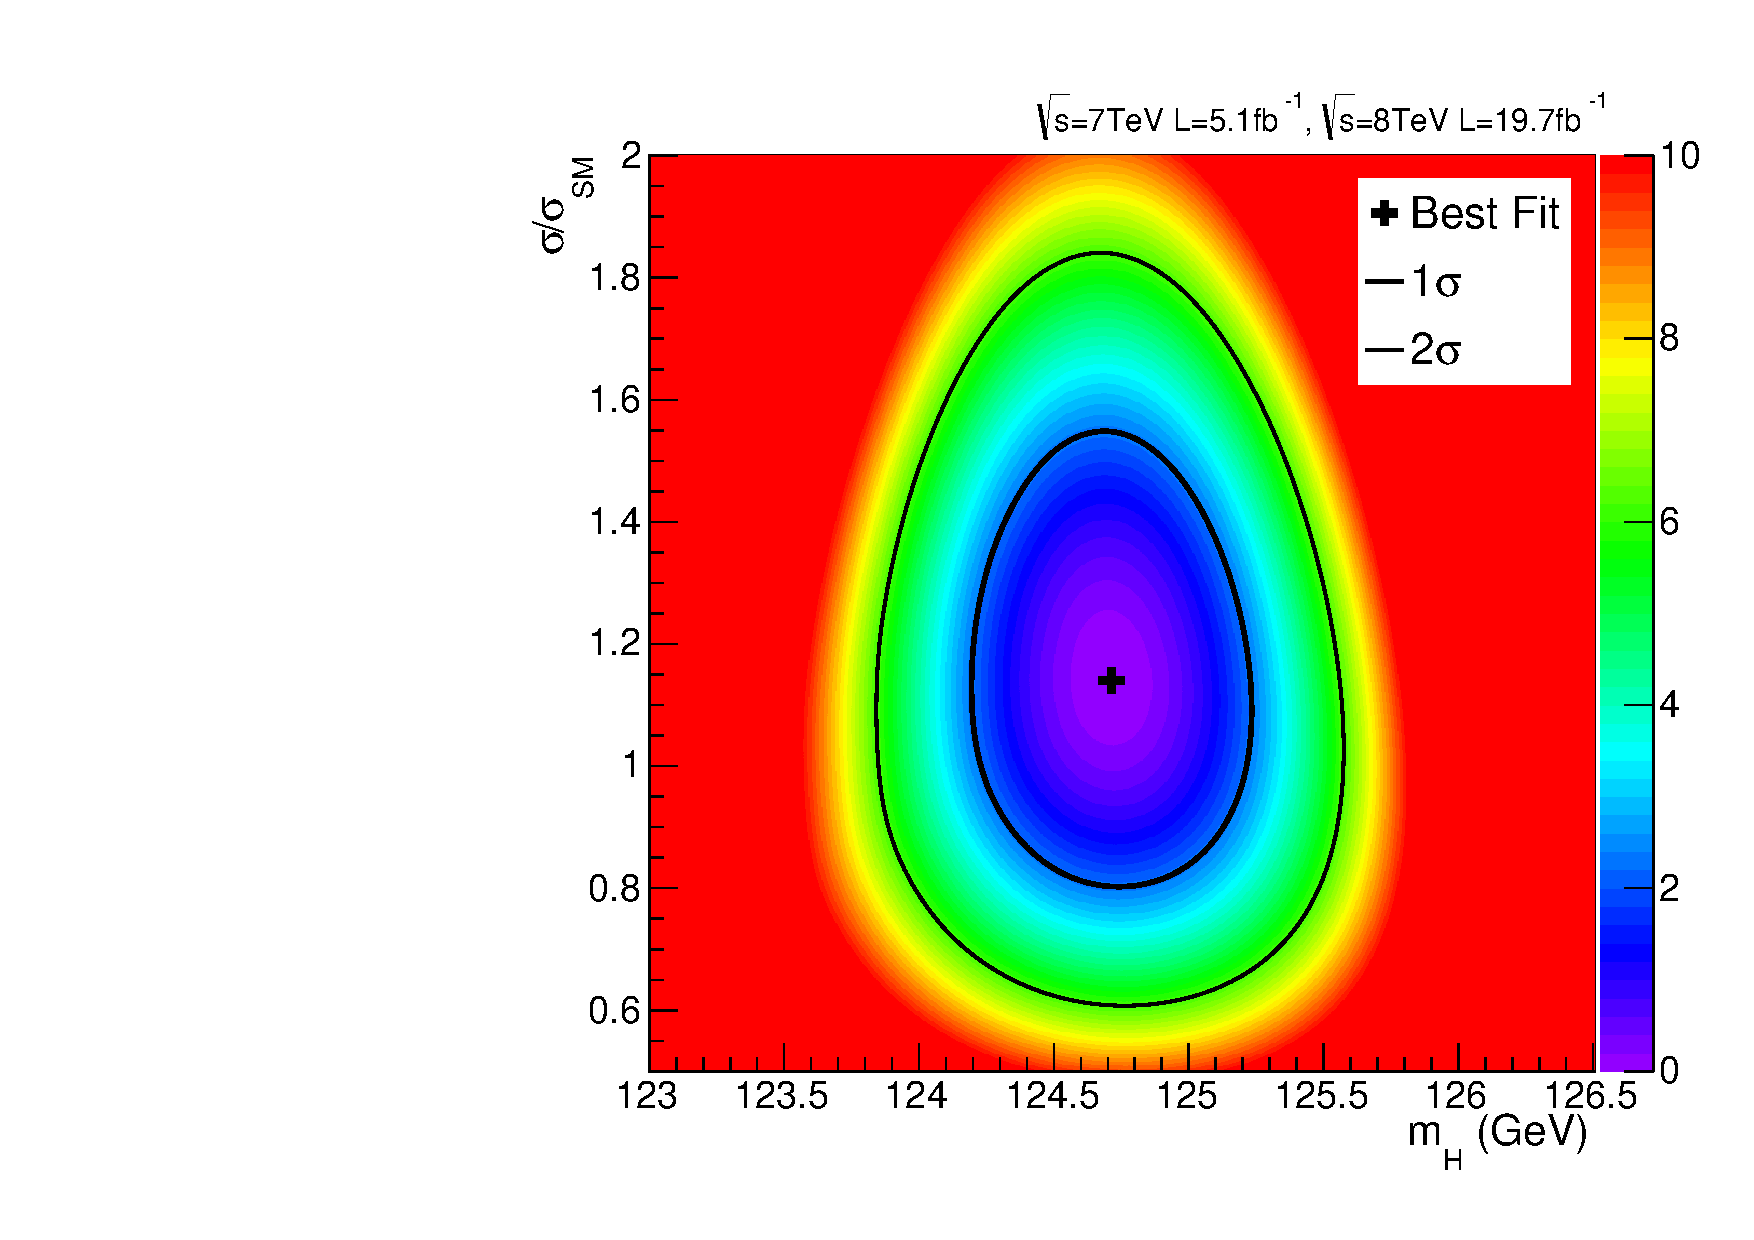
\includegraphics[width=0.49\textwidth]{results/plots/mva_mumh_scan.png}
  \includegraphics[width=0.49\textwidth]{results/plots/mva_mh_scan.pdf}
  \caption[2D \NLL scans of $\mu$ and \mH]{The two dimensional \NLL scan of $\mu$ and \mH when fitting to the combined 7+8~\TeV dataset is shown on the left. The best fit value is shown by the black cross and the $1\sigma$ and $2\sigma$ error contours shown by the solid lines. The one dimensional \NLL scan of the best fit mass \mH is shown on the right, when profiling over the relative signal production from fermionic and bosonic modes, \RF and \RV. The statistical-only component is shown as the blue line and the statistical plus systematic as the black line.}
  \label{fig:res_mumh2}
\end{figure}

Aside from the mass and signal strength of the observed particle it is relevant to study its couplings and whether the relative fractions produced by the different production modes are also compatible with the \SM prediction. This is addressed in Fig.~\ref{fig:res_rvrf}. One-dimensional \NLL scans of the relative couplings to fermions, \RF, and bosons, \RV, are shown in the top right and top left plots respectively. It is clear that the excess of signal in 7~\TeV dataset is apparent in both the fermionic and bosonic production modes, with a large excess in the tight \VBF category at 7~TeV driving the very high value of \RV in the 7~TeV dataset. The slight deficit, with respect to the \SM, in the 8~\TeV dataset comes mainly from the bosonic production modes. Figure~\ref{fig:res_rvrf} also shows the equivalent two dimensional \NLL scan of both of these parameters simultaneously. It can be seen that the observation of $\mu_{ggH,ttH}=1.13^{+0.37}_{-0.31}$, $\mu_{qqH,VH}=1.16^{+0.63}_{-0.57}$ is very compatible with the \SM expectation. Furthermore, the signal strength can be divided by production mode as also shown in Fig.~\ref{fig:res_rvrf}. It can be seen that the signal strength for all four production mechanisms is consistent with the \SM expectation at 1. The Higgs mass, \mH, is profiled in all of these scans but constrained to be the same across each production mode.

\begin{figure}
  \includegraphics[width=0.49\textwidth]{results/plots/mva_rv_scan.pdf}
  \includegraphics[width=0.49\textwidth]{results/plots/mva_rf_scan.pdf} \\
  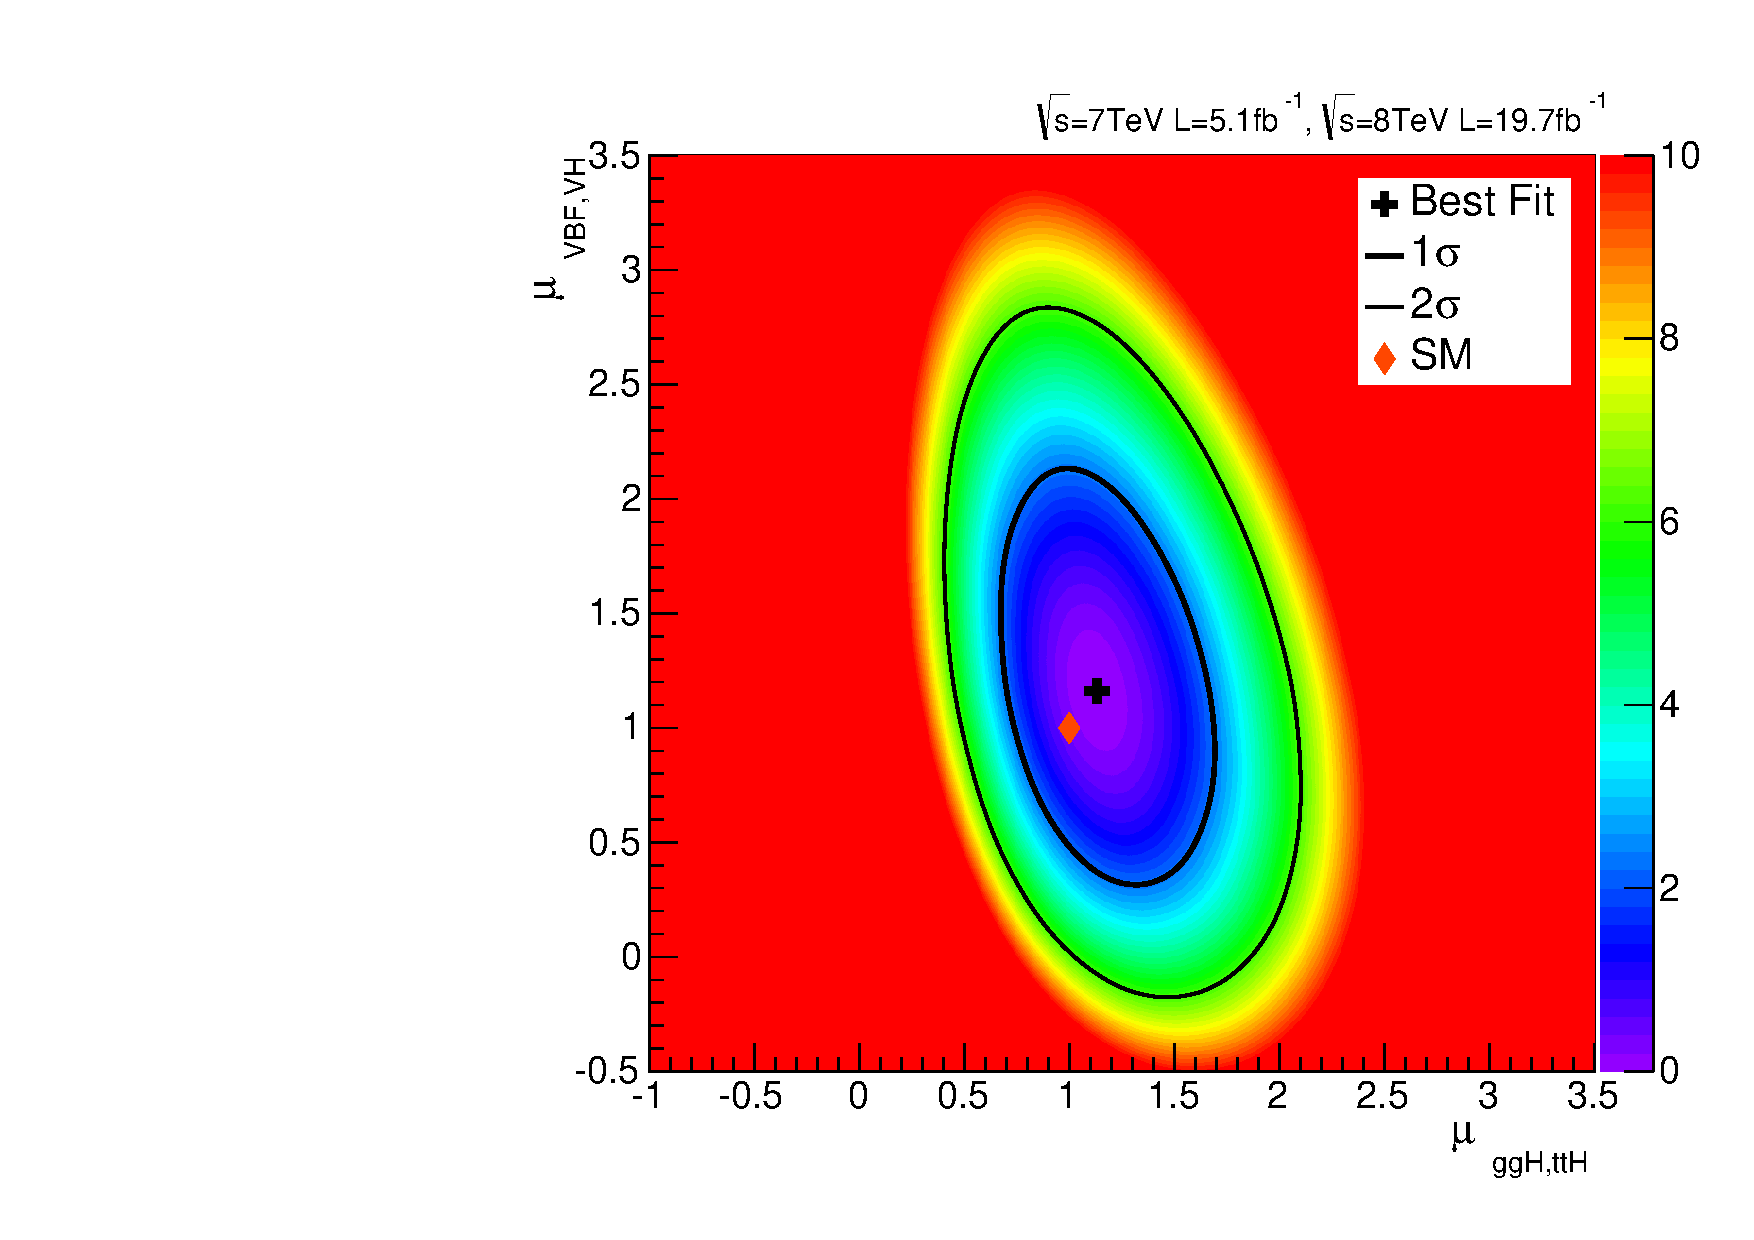
\includegraphics[width=0.49\textwidth]{results/plots/mva_rvrf_scan.png}
  \includegraphics[width=0.49\textwidth]{results/plots/mva_proc_scan.pdf}
  \caption[Best fit values and \NLL scans of the signal strength from fermionic and bosonic production modes]{The top row shows the one dimensional \NLL scan of the \SM relative signal strength from bosonic production modes, $\RV$ (top left), and from fermionic production modes, $\RF$ (top right) for the 7~\TeV (red), 8~\TeV (blue) and combined (black) datasets. The bottom left plot is the 2D \NLL scan of $\mu_{qqH,VH}$ ($y$-axis) vs.~$\mu_{ggH,ttH}$ ($x$-axis) for the combined dataset observation. The best fit point is shown by the black cross whilst the $1\sigma$ and $2\sigma$ error intervals are shown by the solid lines. The \SM expectation is the red diamond. It can be seen that the observation is very compatible with the \SM prediction. The bottom right plot shows the value of the observed signal strength (black points) when floating the separate contributions from each production process with a common mass compared to the combined best fit value (green band). It can be seen that each individual coupling component is compatible with the observation and the \SM expectation. The $\chi^{2}$ $p$-value for this compatibility is $p(\chi^{2})=49\%$.}
  \label{fig:res_rvrf}
\end{figure}

Figure ~\ref{fig:res_chcomp} shows the breakdown of the extracted signal strength when separately fitted for each of the analysis categories and when grouping the categories by their topology into those which are untagged, those which are dijet (or \VBF) tagged, \VH tagged or \ttH tagged. It is noticeable that the categories with the most sensitivity are the untagged categories, especially the ``Untagged 1" and ``Untagged 2" at 8~\TeV, whilst the dijet categories also have considerable sensitivity because the signal to background ratio is high and the statistics are reasonable. The \VH and \ttH tagged categories have the least sensitivity and whilst they do not contribute much to the error on the total signal yield they are important when measuring the couplings of the observed boson.

\begin{figure}
  \includegraphics[width=0.49\textwidth]{results/plots/mva_chcomp.pdf}
  \includegraphics[width=0.49\textwidth]{results/plots/mva_topo_scan.pdf}
  \caption[The observed compatibility of the signal strength between channels]{The left plot shows the signal strength breakdown when fitting the signal strength, $\mu$, in each analysis category separately. The compatibility is found to be $p(\chi^{2})=74\%$. The right plot shows the signal strength breakdown when fitting categories split by their topology (tag type). The compatibility is found to be $p(\chi^{2})=49\%$.}
  \label{fig:res_chcomp}
\end{figure}

\section{Spin}
\label{sec:spin_results}

This section presents results of the spin analysis. The first part concentrates on extracting the differential signal strength, relative to the \SM expectation, as a function of the decay angle, \costhetastar (see Eq.~\ref{eq:costheta}). The second part describes the results of a statistical hypothesis test to exclude particular spin-2 models.

\subsection{SM compatibility check}
The signal yield, $\mu=\sigma/\sigma_{SM}$, is extracted independently in each of the \abscostheta bins, 
simultaneously fitting over the $\eta$ and \rnine bins such that the relative yields in each of the $\eta$ and \rnine 
bins is constrained to that predicted by the SM. The result is shown in Figure~\ref{fig:channelcomp} for the data and various \twomp model expectations, where for the expectations a single representative toy is used, obtained using asymptotic formulae from Ref.~\cite{asymptotic_form}, and the normalisation is extracted from a fit to data. The concept of Fig.~\ref{fig:channelcomp} is to compare the data distribution of \abscostheta to the expectation of various different spin hypotheses. One would expect that the coloured lines on this figure replicate the generator level distributions shown in Fig.~\ref{fig:acc_cuts}. This is the case for the \SM \zerop expectation, however the final point of the \twomp expectations is slightly lower than the generator level distributions suggest. The reason for this is that the efficiency $\times$ acceptance ratio of the \zerop to the \twomp is not flat in this bin, as shown in Fig.~\ref{fig:eff_acc}, which distorts the shape contrary to what might be expected. It can be seen that the data is consistent with being flat. The $\chi^{2}$ compatibility between the data and the \SM expectation is $p(\chi^{2})=86\%$.

\begin{figure}
  \begin{center}
    \includegraphics[width=0.8\linewidth]{results/plots/chcomp.pdf}
    \caption[The \acs{SM} signal strength extraction in bins of \abscostheta for the spin analysis]{The SM extracted signal yield as a function of \abscostheta for the \zerop expectation (red line), \twomp expectation with gluon fusion production only (blue line), the \twomp expectation with quark-antiquark annihilation production only (green line), the \twomp expectation with half $gg$, half $q\bar{q}$ production (magenta line) and the observation (black points).}
    \label{fig:channelcomp}
  \end{center}
\end{figure}

\subsection{Hypothesis tests of the SM Higgs, \zerop, vs. graviton-like, \twomp}
\label{sec:spin_separation}

The separation between either of the two models and the data is extracted using the test statistic, $q$, defined as twice the negative ratio 
of the likelihoods for the \zerop signal plus background hypothesis and the \twomp signal plus background hypothesis when 
performing a simultaneous fit of all forty event classes together, $q=-2\,{\ln({\cal L}_{2^{+}_\mathrm{m} + \mathrm{bkg.}}/{\cal
L}_{0^+ + \mathrm{bkg.}})}$.

The distribution of this test statistic is shown in 
Fig.~\ref{fig:separation} for pseudo-experiments generated with an overall signal yield and signal position which is extracted from a fit to the data for
the \zerop hypothesis 
and the \twomp hypothesis. The $1-CL_{s}$ observed exclusion for a gluon fusion-only produced spin-2 boson is 94\% whilst for quark-antiquark produced boson is 85\%. 

\begin{figure}
  \begin{center}
    \includegraphics[width=0.49\linewidth]{results/plots/2pm0.pdf}
    \includegraphics[width=0.49\linewidth]{results/plots/2pm1.pdf}
    \caption[Distributions of the test statistic for different spin hypotheses compared to the \acs{SM}]{The distribution of the test statistic for pseudo experiments generated under the SM, \zerop, hypothesis (orange) and the \emph{graviton-like}, \twomp, hypothesis (blue) with gluon fusion production only (left) and quark-antiquark production only (right). The observed value in the data is shown as the red arrow.}
    \label{fig:separation}
  \end{center}
\end{figure}

The previous two tests are both performed assuming that the \twomp state is produced entirely by either gluon-fusion or quark-antiquark annihilation. A further three points, with mixtures of $gg$ and $q\bar{q}$ spin-2 production, of 25\%, 50\% and 75\%, have been tested such that the overall yield of the \twomp signal is fixed to the best fit value of the model in question to data and the fraction of \qqbar production is increased by a factor, \fqqbar. Figure~\ref{fig:qqbar} shows the distribution of the test statistic as a function of the fraction of \twomp production from $q\bar{q}$ annihilation. Figure~\ref{fig:separation} is, in effect, a projection of Fig.~\ref{fig:qqbar} at the points $\fqqbar=0\%$ and $\fqqbar=100\%$. It can be seen that the data is very much in line with the \SM expectation. Whilst \textit{a priori} it may look as though the data points in Fig.~\ref{fig:qqbar} lie too close to the \SM mean (red line), all of these points are highly correlated. If the data look flat in \abscostheta then they will look flat for all values of \fqqbar. In this sense the green and yellow bands in Fig.~\ref{fig:qqbar} can be misleading as they do not show these correlations.

\begin{figure}
  \begin{center}
    \includegraphics[width=0.8\linewidth]{results/plots/fqqbar.pdf}
    \caption[Distribution of the test statistic as a function of \fqqbar for the spin analysis]{The distribution of the test statistic for pseudo-experiments generated according to the SM, \zerop, hypothesis (red) and the \emph{graviton-like}, \twomp, hypothesis (blue) as a function of the fraction of \qqbar production relative to $gg$ production. The observed distribution in the data is shown by the black points.}
    \label{fig:qqbar}
  \end{center}
\end{figure}

These results show an independent discovery, in the \Hgg channel alone, of the Higgs like state around 125~\GeV which was announced by the \CMS and ATLAS collaborations in 2012~\cite{CMSDiscovery,ATLASDiscovery}. Furthermore, measurements of the properties of the observed resonance in this decay channel indicate a particle very consistent with the \SM prediction.


